% Перестроение в двумерном случае.
\subsection{Методы перестроения поверхности в двумерном случае}

Рассмотрим геометрическую задачу о перестроении поверхности в двумерном пространстве в общем виде \cite{Rybakov2019Geo2D}.
Пусть даны $n$ ячеек поверхностной сетки, каждая из которых представлена отрезком длины $l_i$ (то есть общее количество узлов равно $n + 1$).
Известно направление изменения поверхности каждой ячейки (направление нормали к отрезку), а также направление движения каждого узла $\overline{g_i}$, $|\overline{g_i}| = 1$.
Оно совпадает с направлением суммы единичных нормалей, проведенных к инцидентным ячейкам.
К тому же для двумерного случая это направление лежит на биссектрисе угла, образованного двумя инцидентными ячейками \cite{Fortin2004Remesh2d} (рис.~\ref{fig:text_1_remesh_2d_grid_normals}).

\begin{figure}[h]
\onelinecaptionstrue
\centering
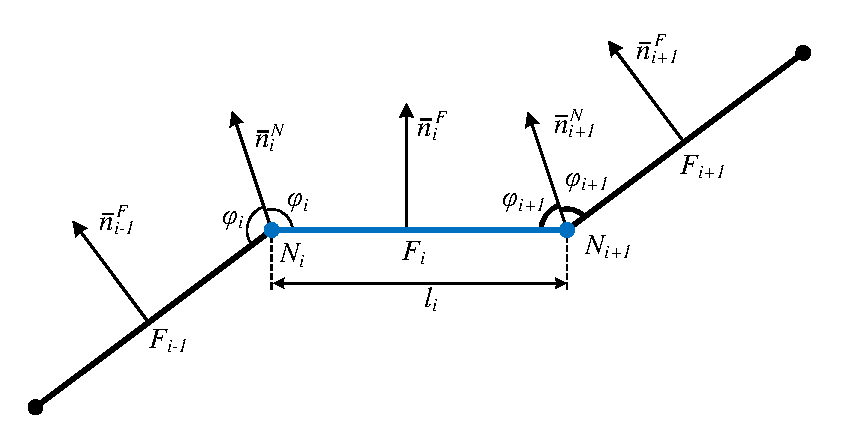
\includegraphics[width=0.7\textwidth]{pics/text_1_remesh_2d/grid_normals.pdf}
\captionstyle{normal}\caption{Поверхностная сетка с обозначенными направлениями движения узлов.}
\label{fig:text_1_remesh_2d_grid_normals}
\end{figure}

Также известны локальные сдвиги поверхности для каждой ячейки (они задаются значениями $H_i$).
Требуется найти такие значения локальных сдвигов узлов сетки $h_i$, чтобы охватывающая площадь между исходной поверхностью и новой поверхностью для каждой ячейки сетки ($S_i$) как можно меньше отличалась от требуемого значения $T_i = l_iH_i$.

Для решения данной задачи сначала требуется вычислить охватываемую площадь для каждой отдельной ячейки.

\subsubsection{Задача о вычислении охватываемой площади при движении узлов отдельной ячейки}

Рассматривается ячейка, представленная на плоскости отрезком $AB$ длины $l$.
При перемещении точек $A$ и $B$ в новые точки $A_1$ и $B_1$ соответственно образуется четырехугольник $AA_1B_1B$.
Требуется найти его площадь, выраженную явно через параметры $a = \overline{AA_1}$ и $b = \overline{BB_1}$ (рис.~\ref{fig:text_1_remesh_2d_local}).

\begin{figure}[h]
\onelinecaptionstrue
\centering
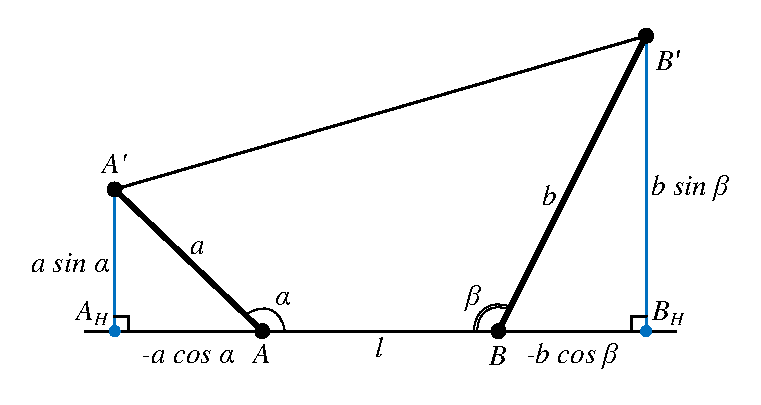
\includegraphics[width=0.7\textwidth]{pics/text_1_remesh_2d/local.pdf}
\captionstyle{normal}\caption{Вычисление охватываемой площади при передвижении узлов ячейки.}
\label{fig:text_1_remesh_2d_local}
\end{figure}

Для решения задачи опустим перпендикуляры из точек $A_1$ и $B_1$ на прямую $AB$.
Их основаниями будут точки $A_2$ и $B_2$ соответственно.
Искомая площадь может быть представлена в следующем виде:
\begin{equation}
S_{AA_1B_1B} = S_{A_2A_1B_1B_2} - S_{AA_1A_2} - S_{BB_1B_2}
\end{equation}

Обозначим угол между векторами $\overline{AA_1}$ и $\overline{AB}$ через $\alpha$, а угол между векторами $\overline{BB_1}$ и $\overline{BA}$ через $\beta$.
Тогда искомая площадь вычисляется явно в следующем виде:
\begin{equation}
S_{AA_1B_1B} = \frac{1}{2}(l - a \cos \alpha - b \cos \beta)(a \sin \alpha + b \sin \beta) + \frac{1}{2}a^2 \sin \alpha \cos \alpha + \frac{1}{2}b^2 \sin \beta \cos \beta
\end{equation}

\begin{equation}
S_{AA_1B_1B} = \frac{1}{2}\big(l(a \sin \alpha + b \sin \beta) - ab \sin(\alpha + \beta)\big)
\end{equation}

\subsubsection{Поиск смещений узлов методом градиентного спуска}

Метод градиентного спуска является одним из наиболее простых методом оптимизации для нахождения локального минимума функции.
При условии, что в любой точки функции можно вычислить ее градиент, то начиная с некоторого начального приближения $x_0$ строится итерационная последовательность~\cite{Kantorovich1984Func}:
\begin{equation}
x^{k+1} = x^k - \gamma_k \nabla f(x_k)
\end{equation}

где $\gamma_k \ge 0$ задает длину шага и, соответственно, скорость градиентного спуска.

Градиентный метод находит свое основное применение в задаче поиска минимума или максимума функции.
Направление антиградиента является направлением наискорейшего убывания функции.
Основная проблема метода заключается в выборе шага $\gamma$.
При слишком больших значениях шага существует вероятность миновать искомый минимум функции.
К тому же, метод не гарантирует нахождение глобального минимума.

Рассмотрим решение поставленной задачи методом градиентного спуска.
Неизвестными параметрами являются величины сдвигов узлов сетки $h_i$ для $0 \le i \le n$.
Опираясь на решение локальной задачи об определении охватываемой площади, можно записать охватываемую площадь при движении отдельной ячейки:
\begin{equation}
S_i = \frac{1}{2}\big(l_i(h_i \sin \alpha_i + h_{i + 1} \sin \beta_i) - h_ih_{i + 1} \sin(\alpha_i + \beta_i)\big) 
\end{equation}

Отклонением охватываемой площади в ячейке от истинного значения будем называть величину $\delta_i = S_i - T_i$, а ошибкой -- ее квадрат $d_i = \delta_i^2$.
Общая ошибка при перестроении поверхности задается как сумма ошибок для всех ячеек:
\begin{equation}
D = \sum_{i = 0}^{n - 1}{d_i}
\end{equation}

При нахождении оптимального решения требуется минимизировать общую ошибку.
Для нахождения градиента требуется вычислить частные производные функции $D$ по всем неизвестным $h_i$.
Эти частные производные можно записать в явном виде:
\begin{equation}
\frac{\partial D}{\partial h_i} = \frac{\partial d_{i - 1}}{\partial h_i} + \frac{\partial d_i}{\partial h_i}
\end{equation}

где
\begin{equation}
\begin{cases}
\frac{\partial d_{i - 1}}{\partial h_i} = \delta_{i - 1}(l_{i - 1} \sin \beta_{i - 1} - h_{i - 1} \sin(\alpha_{i - 1} + \beta_{i - 1})) \\
\frac{\partial d_i}{\partial h_i} = \delta_i(l_i \sin \alpha_i - h_{i + 1} \sin(\alpha_i + \beta_i))
\end{cases}
\end{equation}

\

Также при осуществлении метода градиентного спуска требуется следить за соблюдением дополнительных условий, которые накладываются на неизвестные $h_i$.
Например, очевидным условием является выполнение соотношения $h_i \ge 0$, что запрещает движение сетки в отрицательном направлении.
В нашем случае использовались более строгие условия $\min(H_{i - 1}, H_i) \le h_i \le \max(H_{i - 1}, H_i)$, которые не позволят величинам смещения узлов сетки выходить за пределы смещений инцидентных им ячеек сетки.

\subsubsection{Приближенные методы перестроения поверхности}

Решение задачи о перестроении сетки методом градиентного спуска оказывается слишком требовательным к ресурсам при увеличении размера сетки.
К тому же, качество решения зачастую оказывается неудовлетворительным, особенно при попадании в локальные минимумы.
Поэтому для решения поставленной задачи рассмотрим приближенные методы, основанные на представлении охватываемой площади при движении каждой ячейки с помощью примитивных геометрических фигур.

В качестве первого метода рассмотрим приближение, при котором каждый узел сетки сдвигается на вектор $\frac{1}{2}(H_{i - 1} + H_i)\overline{g_i}$.
Этот метод соответствует представлению площади, охватываемой при движении ячейки длины $l_i$, прямоугольником cо сторонами $l_i$ и $H_i$, а затем выбору в качестве величины смещения узла среднего арифметического высот построенных прямоугольников в инцидентных ячейках, как показано на рис.~\ref{fig:text_1_remesh_2d_grid_rectangles}.

\begin{figure}[h]
\onelinecaptionstrue
\centering
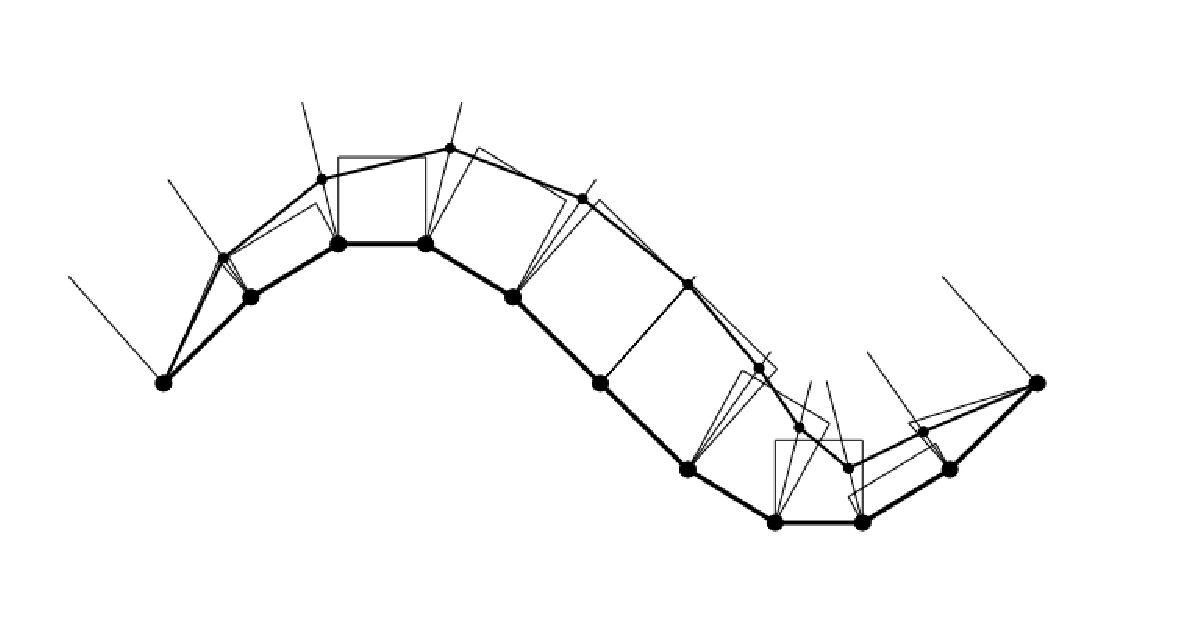
\includegraphics[width=0.7\textwidth]{pics/text_1_remesh_2d/grid_rectangles.pdf}
\captionstyle{normal}\caption{Перестроение поверхности методом прямоугольников.}
\label{fig:text_1_remesh_2d_grid_rectangles}
\end{figure}

В методе трапеций охватываемая площадь при движении ячейки представляется трапецией с площадью $T_i$, боковые стороны которой лежат на направлениях роста двух узлов, относящихся к рассматриваемой ячейке (направения $\overline{g}_{i - 1}$, $\overline{g}_i$).
После построения трапеций для всех ячеек сетки у каждого внутреннего узла появляется две новые потенциальные позиции для сдвига (образованные ячейкой слева и ячейкой справа).
В качестве финальной новой позиции выбирается их среднее значение (рис.~\ref{fig:text_1_remesh_2d_grid_trapeziums}).

\begin{figure}[h]
\onelinecaptionstrue
\centering
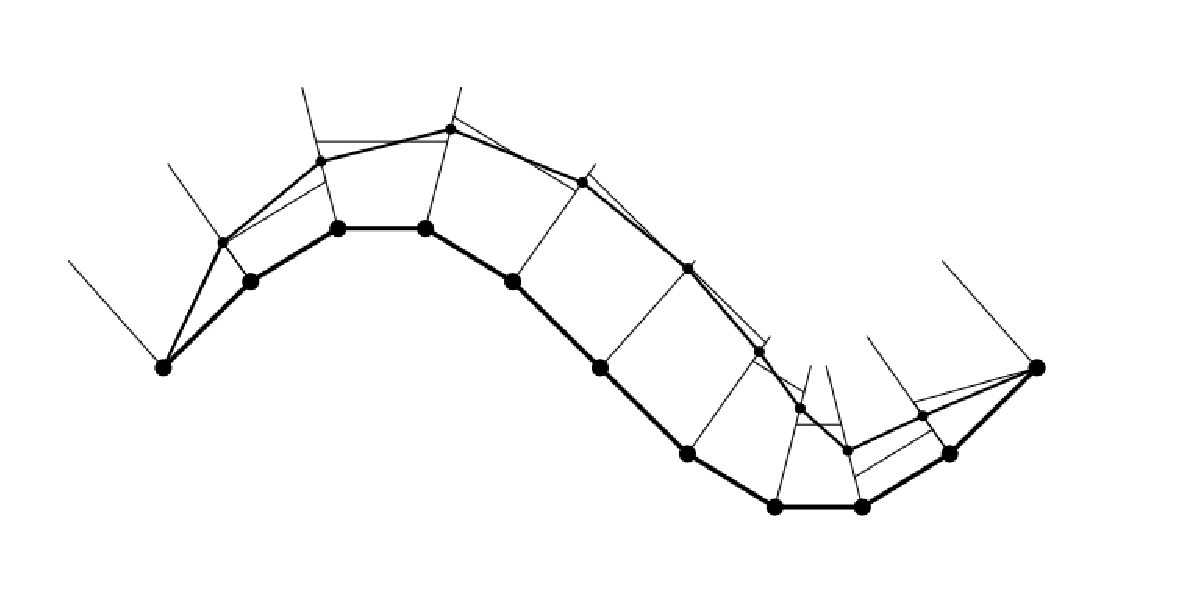
\includegraphics[width=0.7\textwidth]{pics/text_1_remesh_2d/grid_trapeziums.pdf}
\captionstyle{normal}\caption{Перестроение поверхности методом трапеций.}
\label{fig:text_1_remesh_2d_grid_trapeziums}
\end{figure}

Приведем теоретическую оценку точности приближенных методов перестроения поверхности.
Оценку будем производить для модельной расчетной сетки, которая удовлетворяет следующим требованиям.
Все ячейки сетки одинаковые и имеют длину $l$, смещения всех ячеек одинаково и равно $H$, поверхность является выпуклой и кривизна сетки (угол отклонения ячейки от предыдущей ячейки) постоянна и равна $\alpha$ (см. рис.~\ref{fig:text_1_remesh_2d_theoretical_rectangles}).

\begin{figure}[h]
\onelinecaptionstrue
\centering
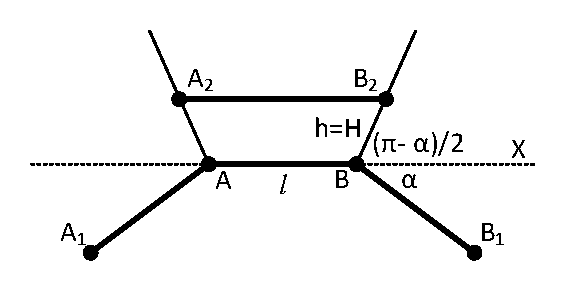
\includegraphics[width=0.6\textwidth]{pics/text_1_remesh_2d/theoretical_rectangles.pdf}
\captionstyle{normal}\caption{Сетка с постоянной кривизной $\alpha$ и постоянным $H$.}
\label{fig:text_1_remesh_2d_theoretical_rectangles}
\end{figure}

Вычислим величину значения $\delta$ для перестроения методом прямоугольников, которая одинаковая для всех ячеек (обозначим ее $\delta_r$).
Для метода прямоугольников величина смещения узла равно смещению в ячейке $h = H$, $\delta_r = S_{AA_2B_2B} - lH$.
Так как для рассматриваемого примера размер ячейки, кривизна сетки и смещение ячейки постоянно, то $AA_2B_2B$ является трапецией.
Для нахождения площади этой трапеции найдем $\angle B_2BX = \frac{\pi + \alpha}{2} - \alpha = \frac{\pi - \alpha}{2}$.
Тогда имеем следующее выражение для величины $\delta_r$:
\begin{equation}\label{eqn:text_1_remesh2_deltar}
	\delta_r = \left( l + H \cos \frac{\pi - \alpha}{2} \right) H \sin \frac{\pi - \alpha}{2} - lH
\end{equation}

\begin{figure}[h]
\onelinecaptionstrue
\centering
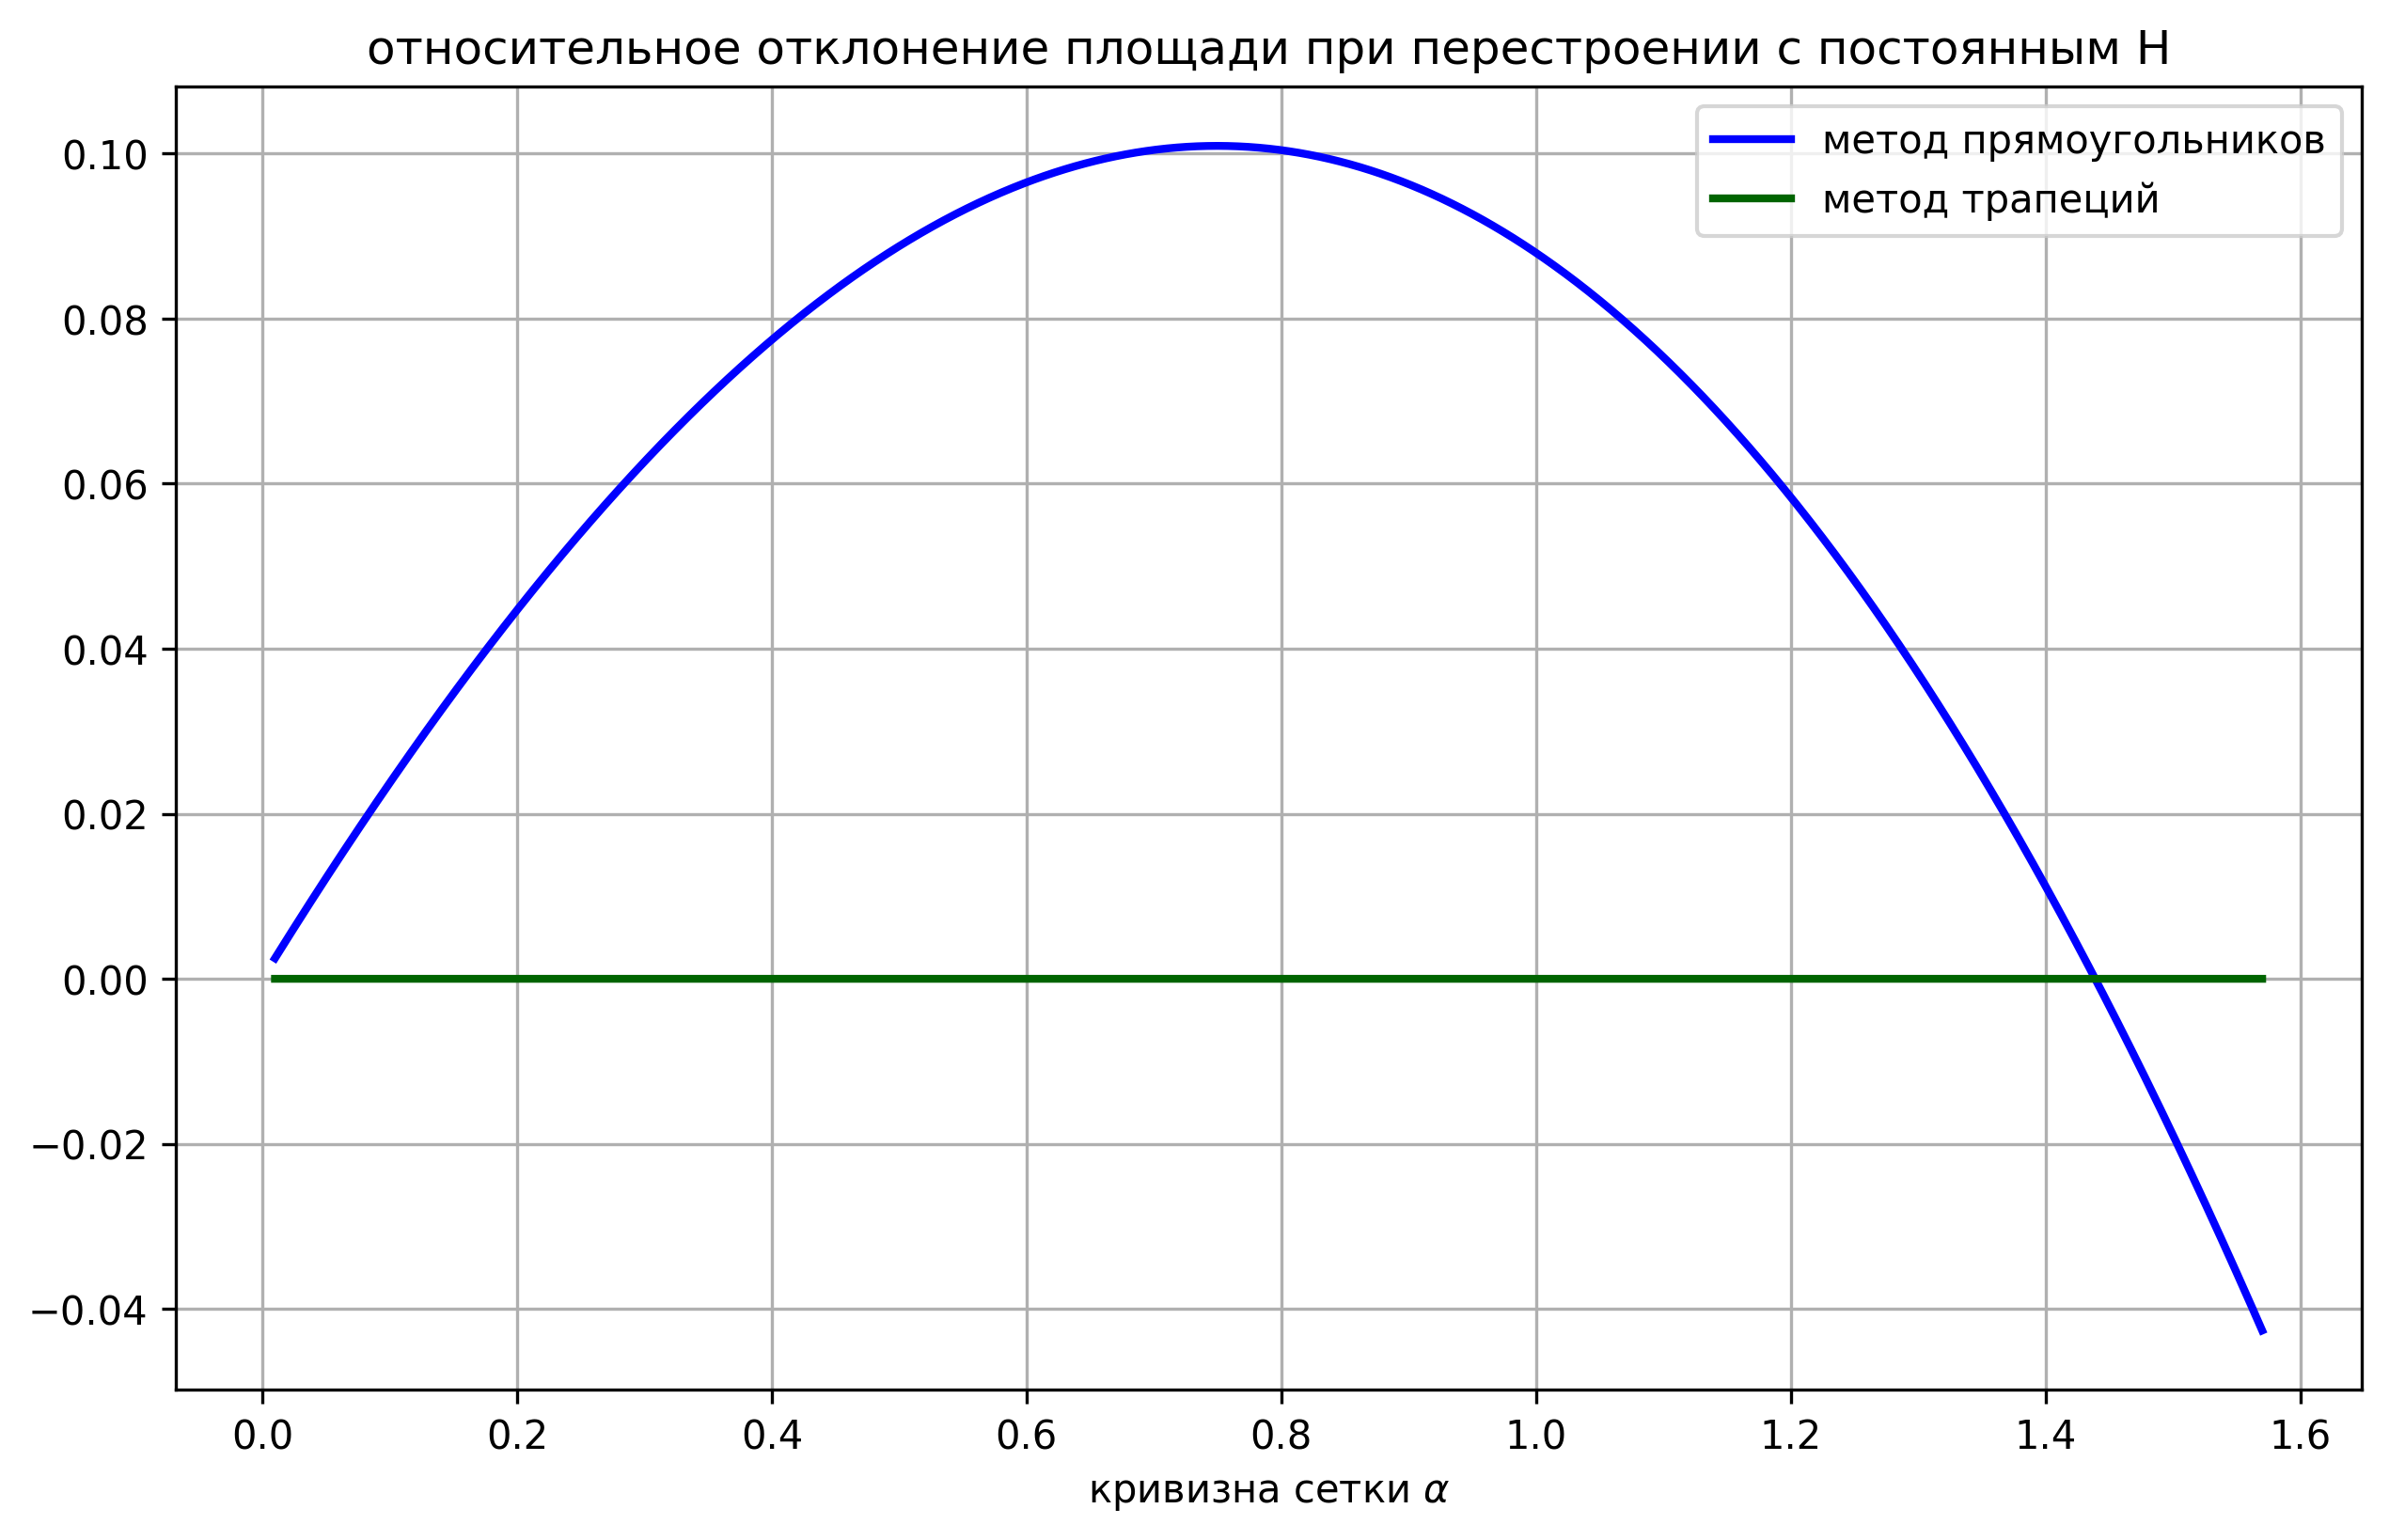
\includegraphics[width=0.7\textwidth]{pics/text_1_remesh_2d/rel_dev_for_const_H.png}
\captionstyle{normal}\caption{Теоретическая оценка относительного отклонение площади $\frac{\delta_r}{lH}$ и $\frac{\delta_t}{lH}$ для сеток с постоянной кривизной и высотой перестроения.}
\label{fig:text_1_remesh_2d_rel_dev_for_const_H}
\end{figure}

Метод трапеций для сеток с постоянными значениями $l$, $H$ и $\alpha$ по своему определению абсолютно точен, то есть в этом случае $\delta_t = 0$.
Результаты теоретических оценок приведены на рис.~\ref{fig:text_1_remesh_2d_rel_dev_for_const_H}.

Теперь возмьмем значение кривизны сетки, при котором перестроение методом прямоугольников демонстируем наихудший результат (это значение примерно равно 0,7).
Проведем анализ отклонения площади при перестроении методом прямоугольников и методом трапеций для сетки с непостоянным значением $H$.

\begin{figure}[h]
\onelinecaptionstrue
\centering
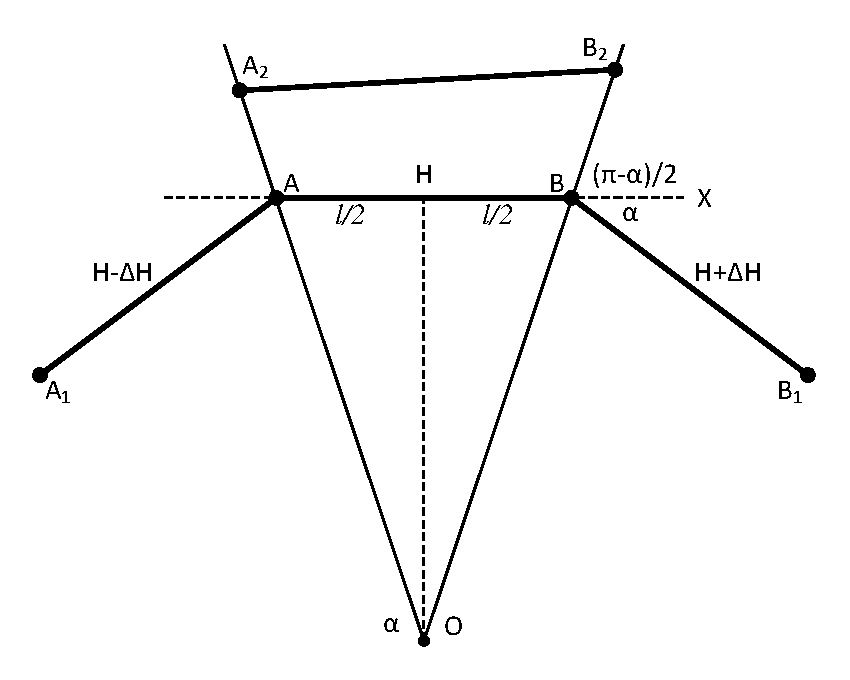
\includegraphics[width=0.6\textwidth]{pics/text_1_remesh_2d/theoretical_rectangles_2.pdf}
\captionstyle{normal}\caption{Сетка с постоянной кривизной $\alpha$ и изменяющимся $H$.}
\label{fig:text_1_remesh_2d_theoretical_rectangles_2}
\end{figure}

Пусть высота перестроения в ячейках у нам не одинаковая, а линейно возрастает при движении по ячейкам.
То есть в рассматриваемой ячейке $AB$ она равна $H$ как и раньше, но в соседних ячейках $A_1A$ и $BB_1$ эта высота равна $H - \Delta H$ и $H + \Delta H$ соответственно (см. рис.~\ref{fig:text_1_remesh_2d_theoretical_rectangles_2}).

Сначала рассмотрим метод прямоугольников перестроения сетки и найдем для него величину $\delta_r$.
Так как $AA_2 = H - \frac{1}{2} \Delta H$, а $BB_2 = H + \frac{1}{2} \Delta H$, и кривизна $\alpha$ постоянна, то $AA_2B_2B$ уже не является трапецией.
С другой стороны при $\alpha > 0$ прямые $AA_2$ и $BB_2$ пересекаются в некоторой точке $O$ и требуемая площадь может быть найдена как $S_{AA_2B_2B} = S_{OA_2B_2} - S_{OAB}$.
Так как треугольник $AOB$ равнобедренный, то $\angle BAO = \angle ABO = \angle B_2BX = \frac{\pi - \alpha}{2}$, а значит $\angle AOB = \alpha$, откуда имеем $OA = OB = \frac{l}{2 \sin \frac{\alpha}{2}}$.
В итоге получим
\begin{equation}
	\begin{aligned}
		& S_{AA_2B_2B} = \frac{1}{2} \sin \alpha \left( \left( OA + \left( H - \frac{1}{2} \Delta H \right) \right) \left( OB + \left( H + \frac{1}{2} \Delta H \right) \right) - OA OB \right) \\
		& S_{AA_2B_2B} = \frac{1}{2} \sin \alpha \left( \frac{lH}{\sin \frac{\alpha}{2}} + H^2 - \frac{1}{4}\Delta H^2 \right)
	\end{aligned}
\end{equation}

Тогда относительное отклонение площади при перестроении методом прямоугольников принимает вид
\begin{equation}
	\delta_r(\alpha, l, H, \Delta H) = \cos \frac{\alpha}{2} \left( lH + \left( H^2 - \frac{1}{4} \Delta H^2 \right) \sin \frac{\alpha}{2} \right) - lH,
\end{equation}

что при $\Delta H = 0$ совпадает с \eqref{eqn:text_1_remesh2_deltar}.

Теперь перейдем к вычислению отклонения $\delta_t$ для метода трапеций.
В методе трапеций мы должн представить охватываемые площади в ячейках $A_1A$, $AB$, $BB_1$ с помощью равнобоких трапеций, для которых известно одно из оснований (одинаково для всех ячеек и равно $l$), угол при другом основании (одинаковый для всех ячеек и равен $\angle B_2BX = \frac{\pi - \alpha}{2}$, а также площади этих трапеций, равные $l(H - \Delta H)$, $lH$ и $l(H + \Delta H)$ соответственно.
На основании этих данных нам необходимо вычислить высоты трапеций, что можно сделать согласно \eqref{eqn:text_1_geo_prim_trapezium_h_from_s}.
Обозначим высоты этих трапеций:
\begin{equation}
	\begin{aligned}	
		& h_t^{A_1A} = h_t^{-} = h\left(\frac{\pi - \alpha}{2}, l, l(H - \Delta H)\right) \\ 
		& h_t^{AB} = h_t = h\left(\frac{\pi - \alpha}{2}, l, lH\right) \\
		& h_t^{BB_1} = h_t^{+} = h\left(\frac{\pi - \alpha}{2}, l, l(H + \Delta H)\right)
	\end{aligned}
\end{equation}

Тогда $AA_2 = \frac{h_t^{-} + h_t}{2 \cos \frac{\alpha}{2}}$, $BB_2 = \frac{h_t + h_t^{+}}{2 \cos \frac{\alpha}{2}}$ и выражение для $S_{AA_2B_2B}$ принимает следующий вид:
\begin{equation}
	\begin{aligned}
		& S_{AA_2B_2B} = \frac{1}{2} \sin \alpha \left( \frac{l (h_t^{-} + 2 h_t + h_t^{+})}{4 \sin \frac{\alpha}{2} \cos \frac{\alpha}{2}} + \frac{(h_t^{-} + h_t)(h_t + h_t^{+})}{4 \cos^2 \frac{\alpha}{2}} \right) \\
		& S_{AA_2B_2B} = \frac{1}{4} \left( (h_t^{-} + 2 h_t + h_t^{+})l + (h_t^{-} + h_t) (h_t + h_t^{+}) \tg \frac{\alpha}{2} \right)
	\end{aligned}
\end{equation}

Тогда отклонение площади от целевого значения при перестроении методом трапеций принимает вид
\begin{equation}
	\delta_t(\alpha, l, H, \Delta H) = S_{AA_2B_2B} = \frac{1}{4} \left( (h_t^{-} + 2 h_t + h_t^{+})l + (h_t^{-} + h_t) (h_t + h_t^{+}) \tg \frac{\alpha}{2} \right) - lH
\end{equation}

\begin{figure}[h]
\onelinecaptionstrue
\centering
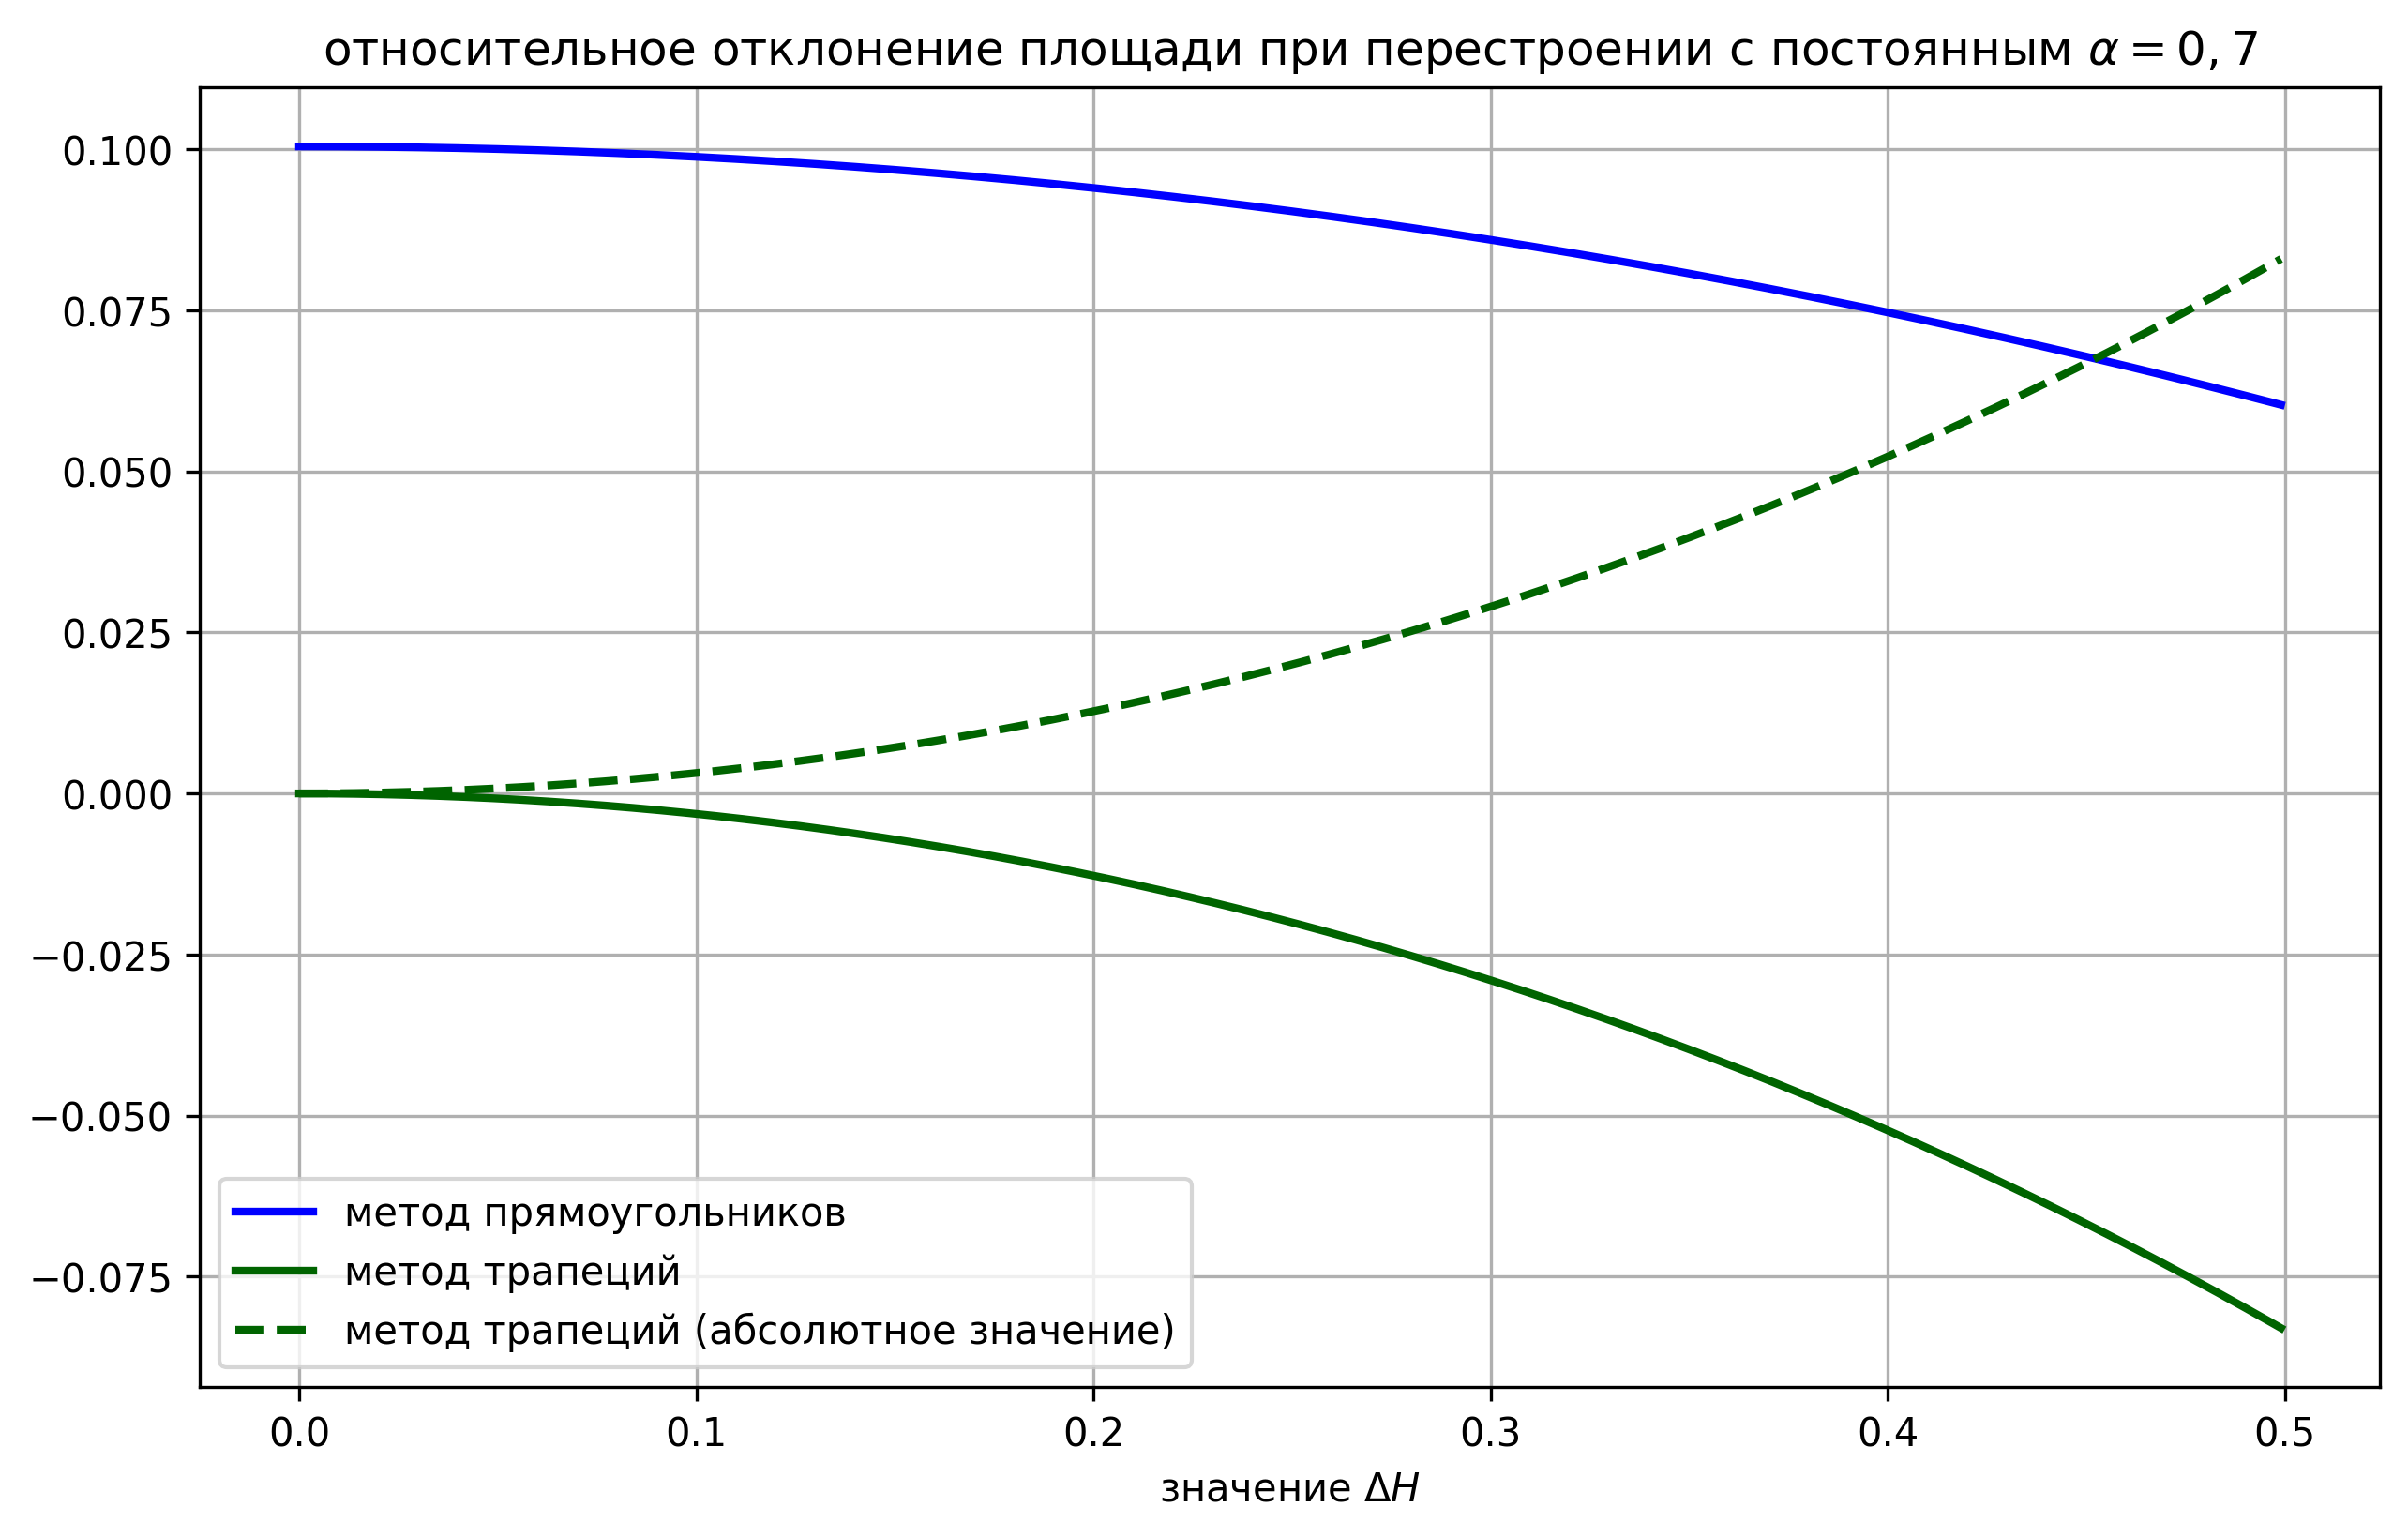
\includegraphics[width=0.7\textwidth]{pics/text_1_remesh_2d/rel_dev_for_const_alpha07.png}
\captionstyle{normal}\caption{Теоретическая оценка относительного отклонение площади $\frac{\delta_r}{lH}$ и $\frac{\delta_t}{lH}$ для сеток с постоянной кривизной и переменным значением $H$ при $\alpha = 0,7$.}
\label{fig:text_1_remesh_2d_rel_dev_for_const_alpha07}
\end{figure}

На рис.~\ref{fig:text_1_remesh_2d_rel_dev_for_const_alpha07} представлены графики относительного отклонения $\frac{\delta_r}{lH}$ и $\frac{\delta_t}{lH}$ площадей при перестроении методом прямоугольников и методом трапеций для $\alpha = 0,7$, размера ячейки $l = 1,0$, высоты перестроения $H = 0,5$ и изменения высоты перестроения $\Delta H \in [0, H]$.
Для метода трапеций дополнительно приведен график абсолютного значения этого отклонения, так как это отклонение отрицательно.
Из приведенных графиков можно сделать вывод, что метод трапеций перестроения является более точным, хотя он несколько затратнее по ресурсам.
